\documentclass[11pt,aspectratio=169]{beamer}
\usepackage[utf8]{inputenc}
\usepackage[T1]{fontenc}
\usepackage{lmodern}
\usepackage[ngerman]{babel}
\usepackage{tikz}
\usetheme{Hannover}

\begin{document}
	\author{Joshua Bär und Michael Steiner}
	\title{Reed-Solomon-Code}
	\subtitle{}
	\logo{}
	\institute{OST Ostschweizer Fachhochschule}
	\date{26.04.2021}
	\subject{Mathematisches Seminar}
	\setbeamercovered{transparent}
	\setbeamertemplate{navigation symbols}{}
	\begin{frame}[plain]
		\maketitle
	\end{frame}
	\section{Einführung}
	\begin{frame}
		\frametitle{Einführung}
		\begin{itemize}
		\item Reed-Solomon-Code beschäftigt sich mit der Übertragung von Daten
		und deren Fehler Erkennung.
		\end{itemize}
	\end{frame}
\section{Polynom Ansatz}
	\begin{frame}
	Beispiel 2, 1, 5 Versenden und auf 2 Fehler absichern.
	\end{frame}
	\begin{frame}
		Übertragen von 
		${f}_2=$\textcolor{blue}{2}, ${f}_1$\textcolor{blue}{1}, ${f}_0$\textcolor{blue}{5} 
		als $ p(w) = \textcolor{blue}{2}w^2 + \textcolor{blue}{1}w + \textcolor{blue}{5} $.
		
		\only<1>{
			Versende $ (p(1),p(2),...,p(7)) = (\textcolor{green}{8}, 
			\textcolor{green}{15}, \textcolor{green}{26},
			\textcolor{green}{ 41}, \textcolor{green}{60}, 
			\textcolor{green}{83}, \textcolor{green}{110})$	
			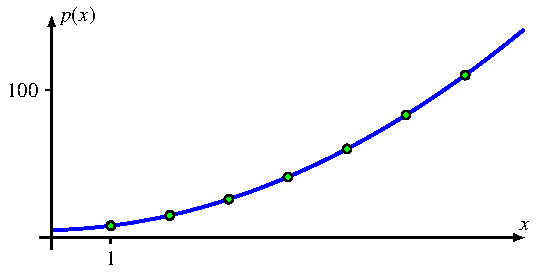
\includegraphics[scale = 1.2]{images/polynom1.pdf}}
		\only<2>{
			Versende $ (p(1),p(2),...,p(7)) = (\textcolor{green}{8}, 
			\textcolor{red}{50}, \textcolor{red}{37},
			\textcolor{green}{ 41}, \textcolor{green}{60}, 
			\textcolor{green}{83}, \textcolor{green}{110})$
			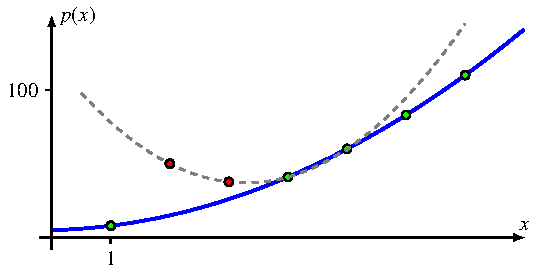
\includegraphics[scale = 1.2]{images/polynom2.pdf}
			\textcolor{green}{7} Zahlen versenden, um \textcolor{blue}{3} Zahlen gegen \textcolor{red}{2} Fehlern abzusichern.}
	\end{frame}

	\begin{frame}
	\frametitle{Parameter}
	\begin{center}
		\begin{tabular}{ c c c } 
			\hline
			"Nutzlast" & Fehler & Versenden \\
			\hline 
			3 & 2 & 7 Werte eines Polynoms vom Grad 2 \\ 
			4 & 2 & 8 Werte eines Polynoms vom Grad 3 \\ 
			3 & 2 & 7 Werte eines Polynoms vom Grad 2 \\ 
			&&\\
			k & t & k+2t Werte eines Polynoms vom Grad k-1 \\ 
			\hline
		\end{tabular}
	\end{center}

	Ausserdem können bis zu 2t Fehler erkannt werden!
	\end{frame}
\section{Fourier Transformation}
	\begin{frame}
		\frametitle{Idee}
		\begin{itemize}
			\item Idee mit Fourier Transformieren und dann senden.
			\item Danach Empfangen und Rücktransformieren.
		\end{itemize}
	\end{frame}

	\begin{frame}
		\begin{figure}
			\only<1>{
			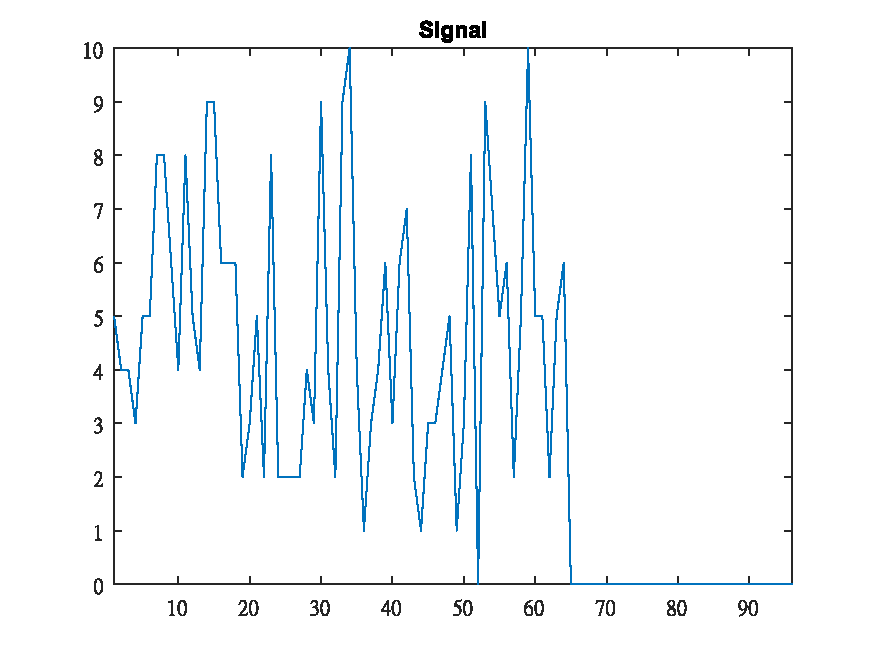
\includegraphics[width=0.9\linewidth]{images/fig1.pdf}
			}
			\only<2>{
			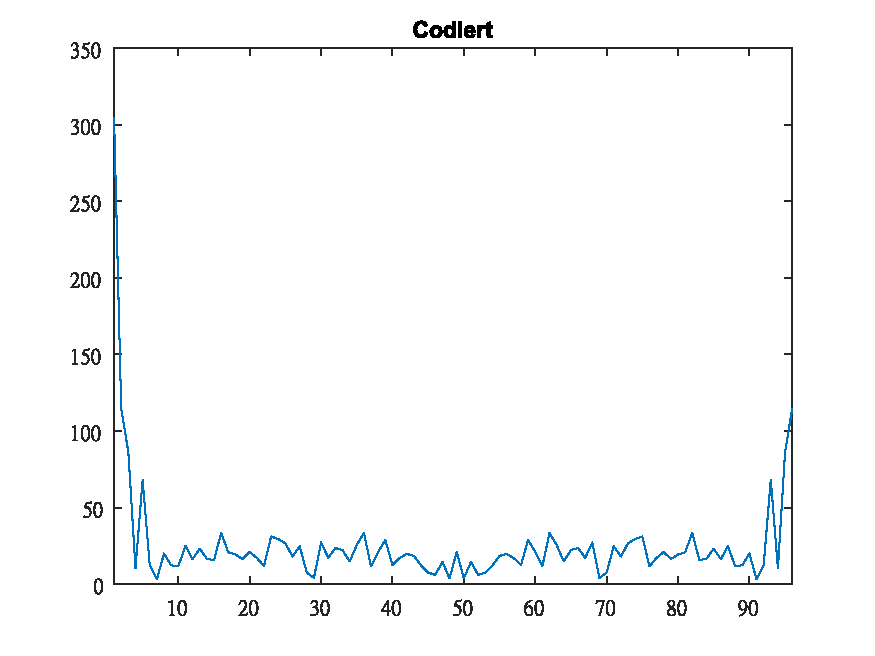
\includegraphics[width=0.9\linewidth]{images/fig2.pdf}
			}
			\only<3>{
			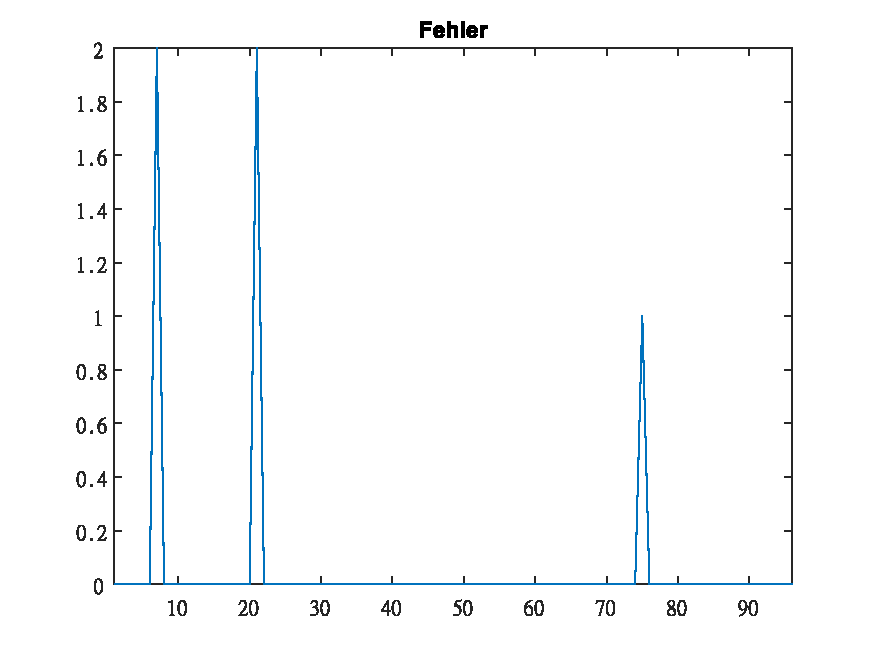
\includegraphics[width=0.9\linewidth]{images/fig3.pdf}
			}
			\only<4>{
			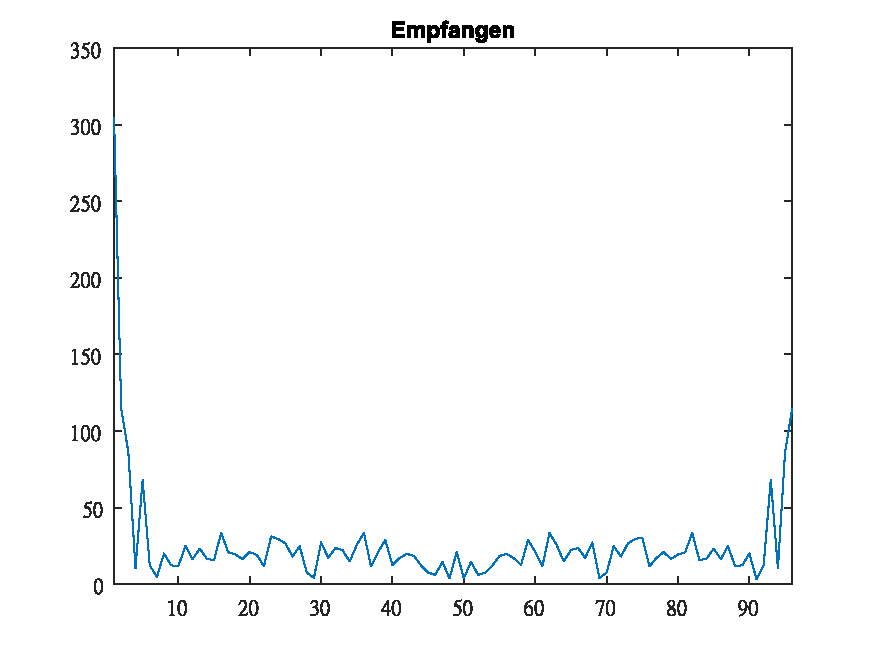
\includegraphics[width=0.9\linewidth]{images/fig4.pdf}
			}
			\only<5>{
			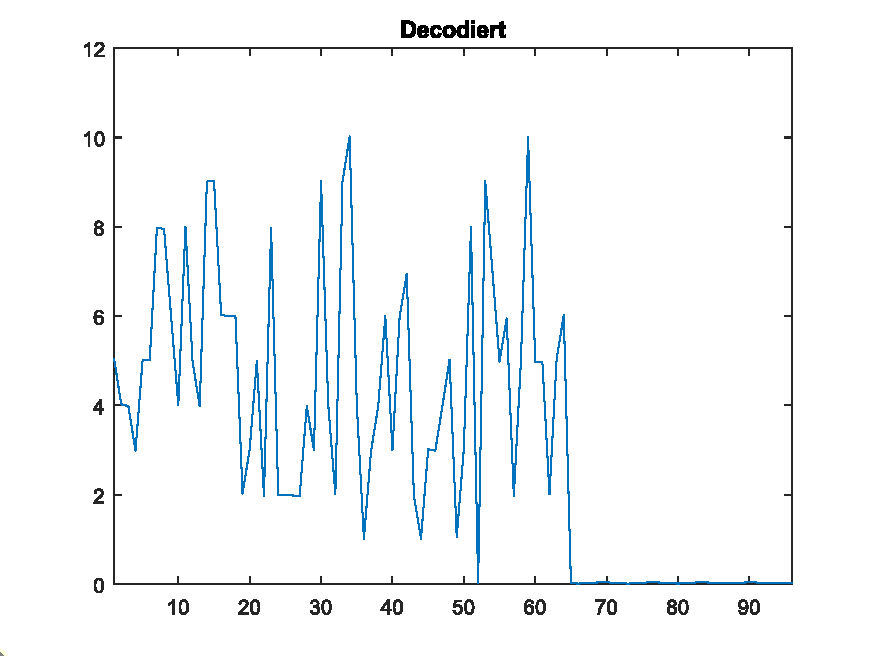
\includegraphics[width=0.9\linewidth]{images/fig5.pdf}
			}
			\only<6>{
			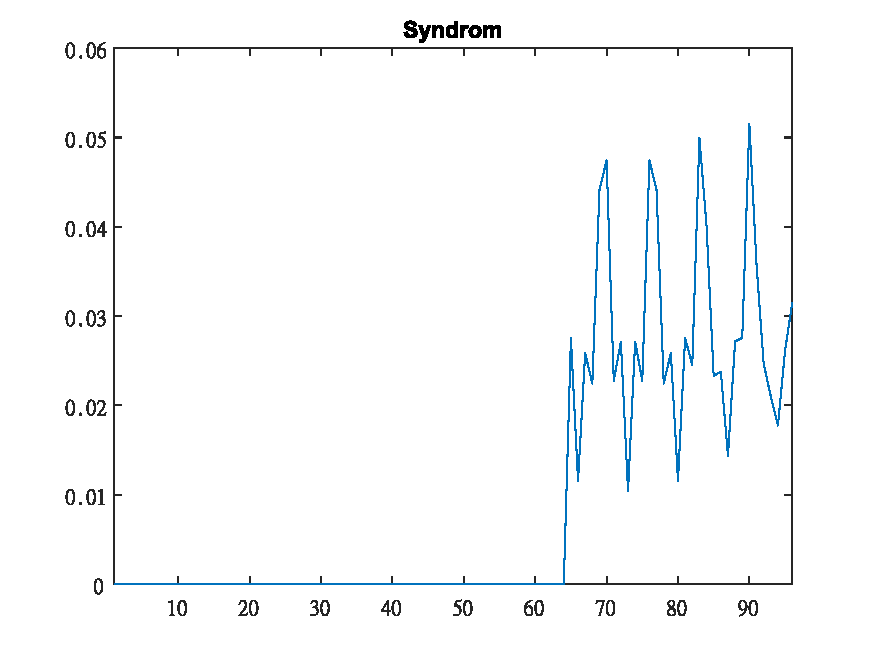
\includegraphics[width=0.9\linewidth]{images/fig6.pdf}
			}
			\only<7>{
			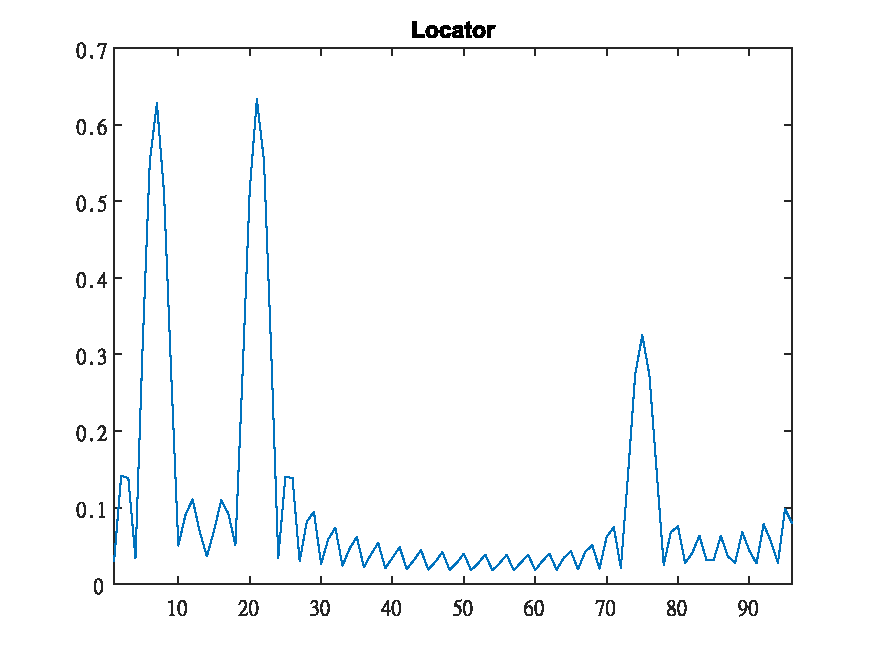
\includegraphics[width=0.9\linewidth]{images/fig7.pdf}
			}
	\end{figure}
	\end{frame}
	
\section{Diskrete Fourier Transformation}
	\begin{frame}
	\frametitle{Diskrete Fourier Transformation}
	Die Diskrete Fourier Transformation ist so gegeben:
	\[
	\label{ft_discrete}
	\hat{c}_{k} 
	= \frac{1}{N} \sum_{n=0}^{N-1}
	{f}_n \cdot e^{-\frac{2\pi j}{N} \cdot kn}
	\].
	
	\[
	w = e^{-\frac{2\pi j}{N} k}
	\]
	Wenn $N$ konstant:
	\[
	\hat{c}_{k}=\frac{1}{N}( {f}_0 w^0 + {f}_1 w^1 + {f}_2 w^2 + \dots + {f}_{N-1} w^N)
	\]
	\end{frame}	


	\begin{frame}
	\frametitle{Diskrete Fourier Transformation}
	\[
	\begin{pmatrix}
		\hat{c}_1 \\\hat{c}_2 \\\hat{c}_3 \\ \vdots \\\hat{c}_n
	\end{pmatrix}
	=
	\begin{pmatrix}
		w^0 & w^0   & w^0  & \dots  &w^0     \\
		w^0 & w^1   &w^2   & \dots  &w^n     \\ 
		w^0 & w^2   &w^4   & \dots  &w^{2n}  \\ 
		\vdots   & \vdots     &\vdots     &\ddots  &\vdots       \\
		w^0 & w^{1n}&w^{2n}& \dots  &w^{n}  \\ 
	\end{pmatrix}
	\begin{pmatrix}
		\textcolor{blue}{f_0}  	\\
		\textcolor{blue}{f_1}	\\
		\textcolor{blue}{f_2}	\\	 
 		\vdots  \\
	 	0  \\ 
	\end{pmatrix}
	\]
	\end{frame}
\section{Probleme und Fragen}
	\begin{frame}
		\frametitle{Probleme und Fragen}
		
			Wie wird der Fehler lokalisiert?
		\only<2>{
			Indem in einem Endlichen Körper gerechnet wird.
		}
	\end{frame}	
\end{document}